% Created 2015-12-26 Sat 12:56
\documentclass[11pt]{article}
\usepackage[utf8]{inputenc}
\usepackage{lmodern}
\usepackage[T1]{fontenc}
\usepackage{fixltx2e}
\usepackage{graphicx}
\usepackage{longtable}
\usepackage{float}
\usepackage{wrapfig}
\usepackage{rotating}
\usepackage[normalem]{ulem}
\usepackage{amsmath}
\usepackage{textcomp}
\usepackage{marvosym}
\usepackage{wasysym}
\usepackage{amssymb}
\usepackage{amsmath}
\usepackage[version=3]{mhchem}
\usepackage[numbers,super,sort&compress]{natbib}
\usepackage{natmove}
\usepackage{url}
\usepackage{minted}
\usepackage{underscore}
\usepackage[linktocpage,pdfstartview=FitH,colorlinks,
linkcolor=blue,anchorcolor=blue,
citecolor=blue,filecolor=blue,menucolor=blue,urlcolor=blue]{hyperref}
\usepackage{attachfile}
\usepackage{pdfcomment}
\usepackage{graphicx}
\usepackage{subfigure}
\date{\today}
\title{org-element-explorer}
\begin{document}

\section{Side by side figures in org-mode}
\label{sec-1}
adapted from \url{http://www.johndcook.com/blog/2009/01/14/how-to-display-side-by-side-figurs-in-latex/}


Now you can reference Figure \ref{fig12}, or Figure \ref{fig:a} or Figure \ref{fig:b}.

\begin{figure}[htb]
\centering
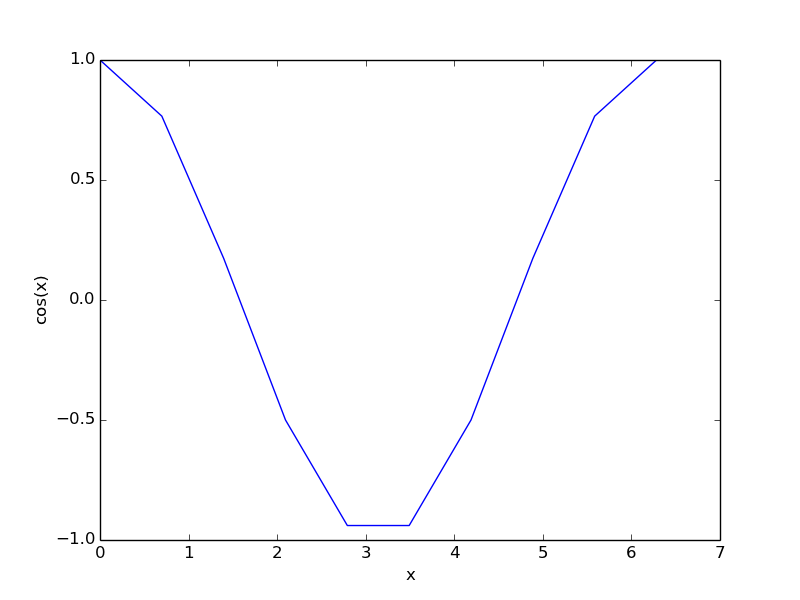
\includegraphics[width=.9\linewidth]{./images/cos-plot.png}
\caption{Left graph \label{fig:a}}
\end{figure}




\begin{figure}
  \subfigure[Left graph \label{fig:a}]
    {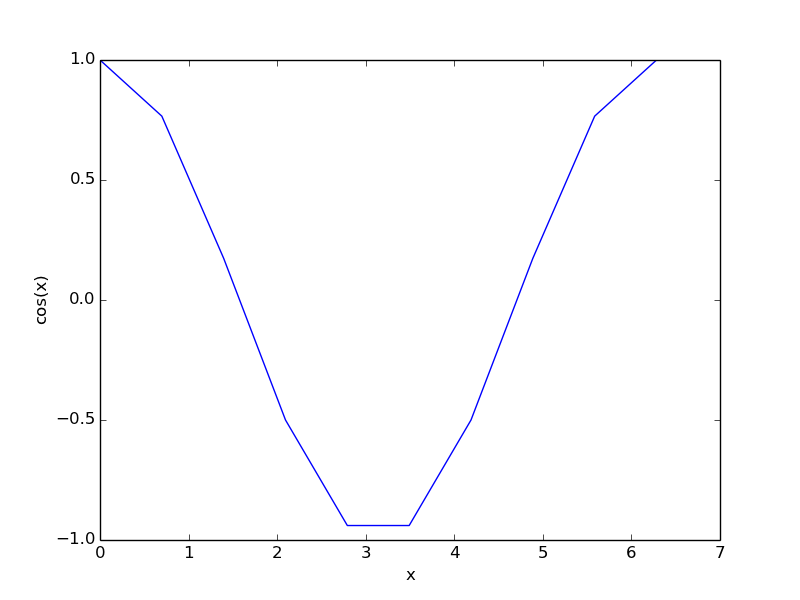
\includegraphics[width=3in]{images/cos-plot.png}}
\enskip % horizontal spacking. tex.stackexchange.com/questions/41476/lengths-and-when-to-use-them
  \subfigure[Right graph. \label{fig:b}]
    {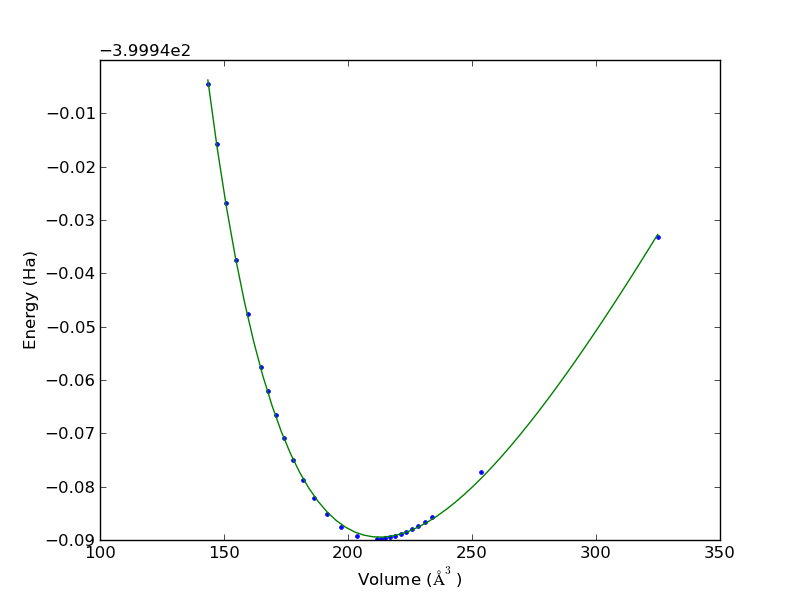
\includegraphics[width=3in]{images/eos-uncertainty.png}}
\caption{Text pertaining to both graphs,\ref{fig:a}and \ref{fig:b}. \label{fig12}}
\end{figure}

Here is an alternative approach we could consider. Kind of like \url{http://oremacs.com/2015/01/23/eltex/}. But we could include other kinds of exports.

\begin{minted}[frame=lines,fontsize=\scriptsize,linenos]{common-lisp}
(figure ()
 (subfigure (("Left graph" (label "fig:a")))
            (includegraphics ((width . "3in"))
                             "images/cos-plot.png"))
 "\enskip"
 (subfigure (("Right graph" (label "fig:b")))
            (includegraphics ((width . "3in"))
                             "images/eos-uncertainty.png"))
 (caption
  "Text pertaining to both graphs, " (ref "fig:a")
  " and " (ref "fig:b") "." (label "fig12")))
\end{minted}

\begin{minted}[frame=lines,fontsize=\scriptsize,linenos]{common-lisp}
(defun label (arg)
  (format "\\label{%s}" arg))

(defun ref (arg)
  (format "\\ref{%s}" arg))

(defun caption (&rest body)
  (format "\\caption{%s}"
         (mapconcat 'eval body "")))

(caption
  "Text pertaining to both graphs, " (ref "fig:a")
  " and " (ref "fig:b") "." (label "fig12"))
\end{minted}
\begin{verbatim}
\caption{Text pertaining to both graphs, \ref{fig:a} and \ref{fig:b}.\label{fig12}}
\end{verbatim}


\begin{minted}[frame=lines,fontsize=\scriptsize,linenos]{common-lisp}
(defun includegraphics (options path)
  (format "\\includegraphics%s{%s}"
          (if options
              (format "[%s]"
                      (mapconcat (lambda (ccell)
                                   (format "%s=%s"
                                           (car ccell)
                                           (cdr ccell)))
                                 options
                                 ","))
            "")
          path))

(includegraphics '((width . "3in"))
                 "images/eos-uncertainty.png")
\end{minted}
\begin{verbatim}
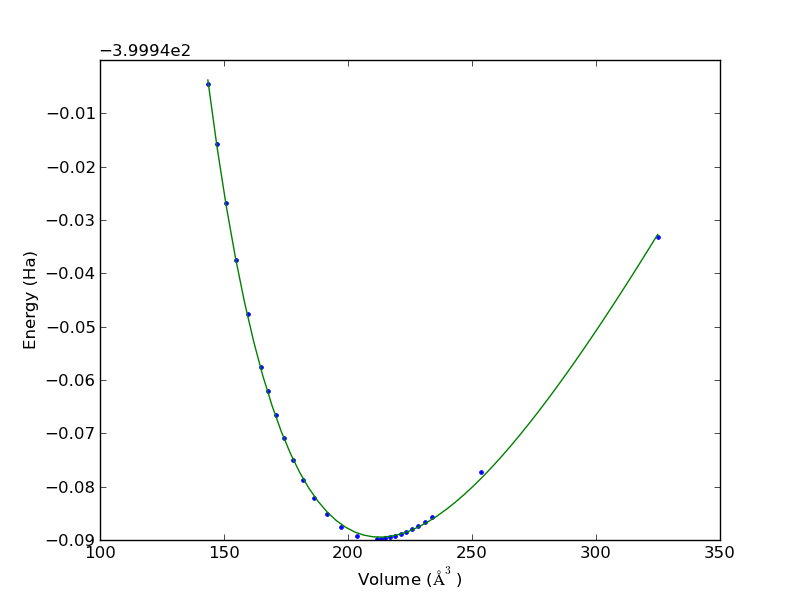
\includegraphics[width=3in]{images/eos-uncertainty.png}
\end{verbatim}

\begin{minted}[frame=lines,fontsize=\scriptsize,linenos]{common-lisp}
(defun subfigure (options &rest body)
  (format "\\subfigure%s{%s}"
          (if options
              (format "[%s]"
                      (mapconcat 'eval options ""))
            "")
          (mapconcat 'eval body "")))

(subfigure '("Right graph" (label "fig:b"))
            (includegraphics '((width . "3in"))
                             "images/eos-uncertainty.png"))
\end{minted}
\begin{verbatim}
\subfigure[Right graph\label{fig:b}]{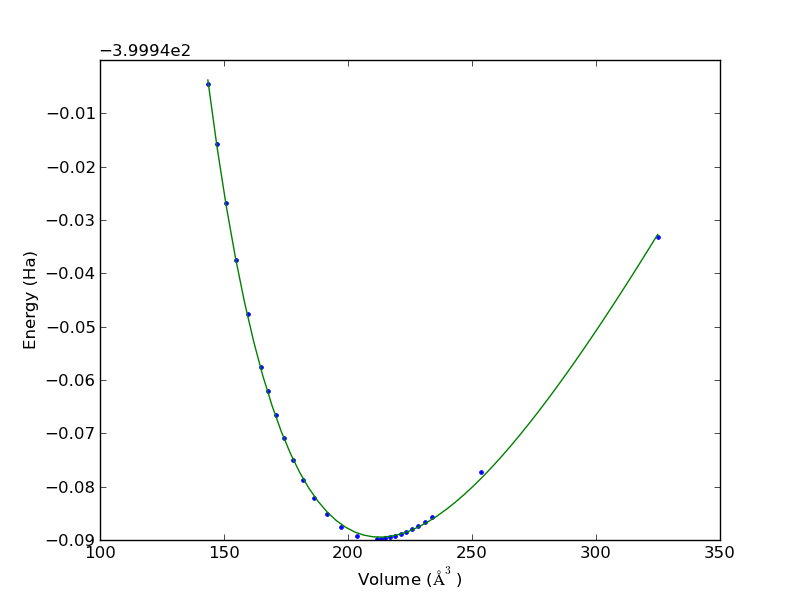
\includegraphics[width=3in]{images/eos-uncertainty.png}}
\end{verbatim}

\subsection{Figure}
\label{sec-1-1}
\begin{minted}[frame=lines,fontsize=\scriptsize,linenos]{common-lisp}
(defun figure (options &rest body)
  (format "\\begin{figure}
%s
\\end{figure}"
(mapconcat 'eval body "\n")))

(figure ()
 (subfigure '("Left graph" (label "fig:a"))
            (includegraphics '((width . "3in"))
                             "images/cos-plot.png"))
 "\\enskip"
 (subfigure '("Right graph" (label "fig:b"))
            (includegraphics '((width . "3in"))
                             "images/eos-uncertainty.png"))
 (caption
  "Text pertaining to both graphs, " (ref "fig:a")
  " and " (ref "fig:b") "." (label "fig12")))
\end{minted}
\begin{figure}
\subfigure[Left graph\label{fig:a}]{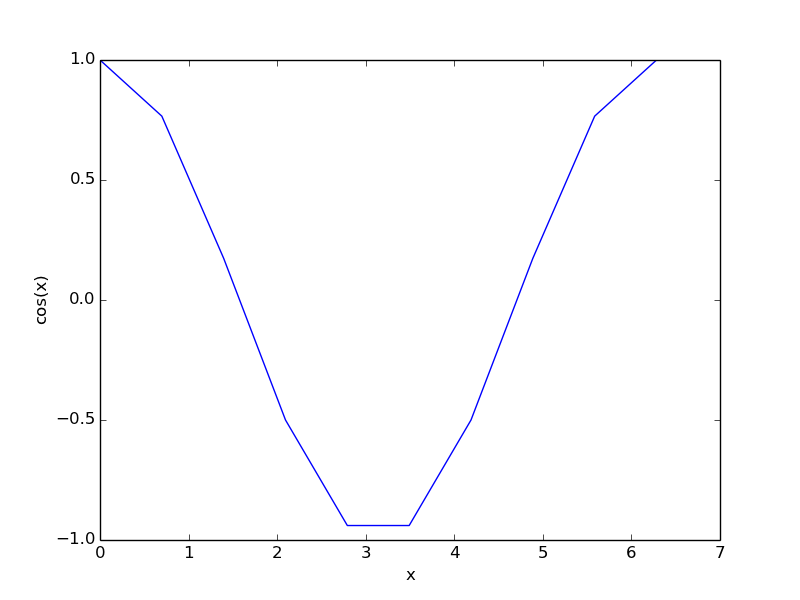
\includegraphics[width=3in]{images/cos-plot.png}}
\enskip
\subfigure[Right graph\label{fig:b}]{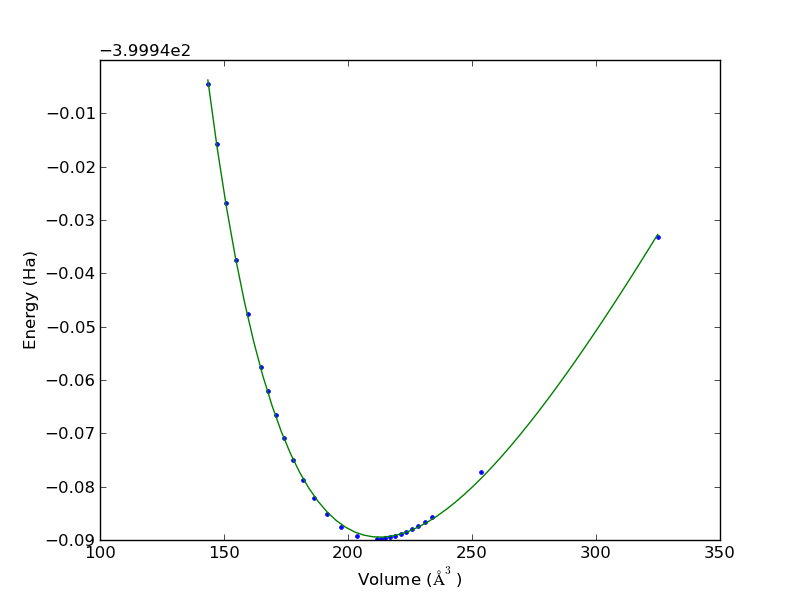
\includegraphics[width=3in]{images/eos-uncertainty.png}}
\caption{Text pertaining to both graphs, \ref{fig:a} and \ref{fig:b}.\label{fig12}}
\end{figure}
% Emacs 25.0.50.1 (Org mode 8.2.10)
\end{document}